
\chapter{Metod2/Genomförande2: Skapandet av läromaterialet}
\begin{draft}

Arbetet med att skapa läromaterialet har haft ett antal delvis parallella faser. Den första fasen (1) var att skapa läromaterial till separata områden inom fysik. Den andra fasen (2a) var att kombinera de tidigare DSLerna till komposita områden. Den tredje fasen (2b) var att använda tidigare DSLer och tillämpa på fysikaliska problem. Den fjärde fasen (2c) var att publicera läromaterial på en hemsida.

Den första fasen var tvunget att ske innan någon annan, då de andra beror på den första. Men efter att lite olika fristående DSLer skapats kunde de tre andra faserna börja ske parallellt. Men den första fasen fortsattae. Olika medlemmar i gruppen arbetade med olika faser samtidigt.

\section{Fas 1: Läromaterial för separata områden}

Processen med att skapa läromaterial för separata områden har varit en loopande process. \ref{fig:oeaversikt_separata} visar en översikt över processen med att skapa läromaterial för de separata områden. Som figuren visar har processen itererat fram och tillbaka mellan de två huvudsakliga stegen selektion och skrivande.

\begin{figure}
  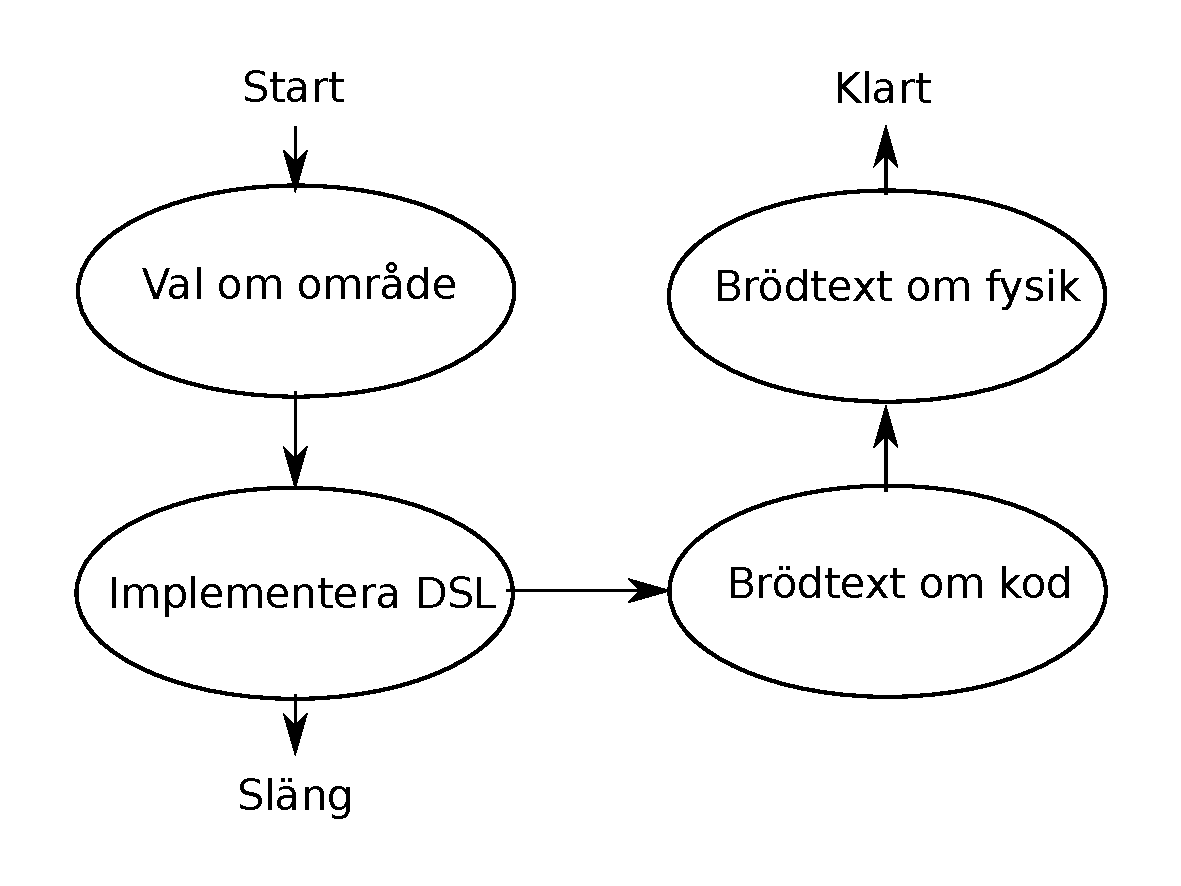
\includegraphics[width=\linewidth]{figure/oeversikt_metod_process.pdf}
  \caption{Översikt över processen med att skapa de separata områdena.}
  \label{fig:oeversikt_separata}
\end{figure}

\todo{Snygga till figuren.}

\subsection{Selektion av områden}

Att hitta områden att arbeta med inom fysik var inget trivialt att göra. De främsta källorna till inspiration var kursboken och annat material som tillhörde kursen. Ett område skulle vara fristående från andra områden, vara grundläggande samt vara ''lämpligt''.

Vad för slags områden detta var, var inget som gick att se bara genom att titta på det. Istället fick det experimenteras med området för att upptäcka om det var ''lämpligt'', dvs gick att representera på ett lätthanterligt och bra sätt i datorn. Dessa krav specifiefas närmare i resultat-kapitelt (då vi visste vad dessa karaktäristika var).

I samband med experiment med DSL skedde också en del inläsning, av bland annat Haskell och Agda. Ett exempel var typnivå-programmering. Detta gjordes för att kunna göra DSL:et på bästa sätt.

Långt ifrån alla försök med områden blev lyckade. Märktes att ett område inte skulle bli något bra DSL så började vi om processen med att hitta ett nytt område. Som tidigare nämnt, så står det vad som var ett bra område och vad som var ett dåligt senare i resultat-kapitlet.

Sökandet efter ett område har utförsts flera gånger i projeket. Ofta skedde det individuellt då. Ett speciellt fall av sökande är dock den initiala selektionen, som skedde i början av projektfasen. Då lästes hela kursboken och allt innehåll radades upp och sorterades. På detta sätt kunde några initiala områden väljas ut att arbteras med. Dessa områden blev

\begin{itemize}
  \item Vektorer
  \item Dimensioner
  \item Momentan och genomsnitt
  \item Differentialkalkyl
\end{itemize}

\subsection{Skrivande av områden}

När ett område verkat fruktsamt och en tanke om hur ett DSL kan se ut börjat formats, så påbörjades en ordentlig implementation av DSL:et. DSLet implementerades i en nästan fullständig utsträckning innan något annat på området gjordes, för att vara säkra att området verklig var lämpligt att göra. Ibland visade det sig, trots de inledande experimenten indikerrade så, att området inte var bra. Då skrotades området.

När hela DSLet var implementerat, ofta med nödtorftiga kodkommentarer, började brödtext som förklarade kod-delen skrivas. Detta var det efterföljande steget för att förstå koden är viktigt, och är ett krav för att man ska kunna skriva en förklaring (och förstå den) om kopplingen till fysik.

Det sista steget är att skriva brödtexten som gör kopplingen mellan DSL och fysik. När själva koden var på plats skrevs hur den relaterar till och modellera fysik. I slutändan skrevs också inledning och avslutning till kapitlet.

\end{draft}
\begin{binge}
\section{Fas 2a: Läromaterial för komposita områden}

Importera DSLerna för varandra för att göra mer komplicerade grejer.

Eller, \emph{Bruk av de mer fundamentala/teoretiska DSLerna för att
  angripa områden av mer ``tillämpad'' natur (såsom Krafter, Arbete,
  etc) )}(?)

!! Områden/moduler soom bygger vidare på redan implementerade områden.

stack, git kan säkert passa här för att beskriva hur vi samarbetade med sammanfogningen.

Selektionen gick till som...

Processen med att skriva läromaterialet gick till på samma sätt som för de separata områdena. Se de kapitlet.

\todo{Här har vi inte gjort så mycket än eller?}

\section{Fas 2b: Tillämpning av DSL:er för problemområden}

Vari vi visar att DSLerna både är praktiskt användbara, likt Wolfram
Alpha, och att implementationen+applikationen hjälper oss förstå
mekanik i allmänhet och probleminstanserna i synnerhet.

% TODO: Motivera varför vi valde LHS
% TODO: Motivera varför vi valde hemsida istället för PDF.
% TODO: Motivera varför vi valde Markdown istället för LaTeX i LHS filerna.

Fritt fall, lutande plan...

Selektion genom...

Skrivande på samma sätt som för separata områden.

\section{Fas 2c: Publicering på hemsidan}

Först en inledande konstruktion av hemsidan.

Sedan löpande att material kompileras och läggs där.

\end{binge}
